%\documentclass[hyperref={pdfpagelabels=false}]{beamer}
%\documentclass[notes=only,xcolor=svgnames,professionalfonts,lualatex]{beamer}
\documentclass[notes=hide,xcolor=svgnames,professionalfonts,lualatex]{beamer}
\mode<presentation>
{
 \usetheme{Dublin} 
}
\usepackage[british]{babel}
\usepackage{fontspec}
\usepackage{mathtools}
\usepackage{listings}
\usepackage[math-style=french,bold-style=upright, nabla=upright,warnings-off={mathtools-colon}]{unicode-math}%
\usepackage{soul}
\usepackage{extramath}
\usepackage{tikz}%
\usetikzlibrary{chains,matrix,positioning,scopes,shapes,shadows,pgfplots.groupplots,decorations.pathmorphing}
\usetikzlibrary{arrows, decorations.markings,fadings}
\usepackage{pgfplots}
\pgfplotsset{compat=newest}
\usepackage{chemarrow}
%\usepackage[final]{movie15}
\usepackage{setspace}
%\usepackage{media9}
\usepackage{pgfpages}
\usepackage{minted}
\uselanguage{BritishEnglish}
\pgfplotsset{compat=newest}
\usepackage[absolute,overlay]{textpos}

\AtBeginDocument{
\setmathfont{New Euler}%
\fontspec[OpticalSize=15]{New Euler}%
\setmainfont[ItalicFont={OpenSans Light Italic},BoldFont={OpenSans},
            BoldItalicFont={OpenSans Italic},Ligatures=TeX]{OpenSans Light}%
\setsansfont[ItalicFont={OpenSans Light Italic},BoldFont={OpenSans},
            BoldItalicFont={OpenSans Italic},Ligatures=TeX]{OpenSans Light}%
\setmonofont[ItalicFont={OpenSans Italic},BoldFont={OpenSans Bold},
            BoldItalicFont={OpenSans Bold Italic},Ligatures=TeX]{OpenSans}%
\setmathfont[range=\mathup/{latin,Latin,num}]{OpenSans Light}%
\setmathfont[range=\mathup/{greek,Greek}]{OpenSans Light}%
\setmathfont[range=\mathbb/{latin,Latin,num}]{OpenSans }%
\setmathfont[range=\mathbf/{latin,Latin,num}]{OpenSans }
\setmathfont[range=\mathbfup/{latin,Latin,num}]{OpenSans }
\setmathfont[range=\mathbfit/{latin,Latin,num}]{OpenSans Italic}
\setmathfont[range=\mathit/{latin,Latin,num}]{OpenSans Light}
\setmathfont[range=\mathtt/{latin,Latin,num}]{OpenSans}
\setmathfont[range=\mathrm]{OpenSans Light}
\setmathfont[range=\mathsfit/{latin,Latin,num}]{OpenSans Light}
\setmathfont[range=\mathsf/{latin,Latin,num}]{OpenSans Light}
\setmathfont[range={"002C,"0021,"003A,"003B,"220F,"2206,"2202}]{OpenSans Light}
\setmathfont[range={"226A,"226B,"00B0,"03F5,"299E,"03D5,"2218,"2221}]{Asana Math}
\setmathfont[range={\mathcal,\mathbfcal,\mathscr},Scale=1.04]{New Euler}
\setmathfont[range={"03B1,"03B3,"2211,"220F,"2212,"002B}]{New Euler}
\DeclareMathSizes{12}{12}{9}{7}
}

%\setbeameroption{show notes on second screen=right}
\graphicspath{{figures/}}
%\setbeamertemplate{navigation symbols}{}
\setbeamertemplate{sidebar right}{}% or get rid of navigation entries there somehow from the default position... 
%\setbeameroption{show notes on second screen}
\newcommand{\captionfont}{\footnotesize}
\title[Metaprogramming, an Introduction]
{Meta-programming, an Introduction}
\author[Christian Lalanne \emph{et. al}] % (optional, use only with lots of authors)
{\textcolor{CherryRed}{Christian Lalanne}}
% - Give the names in the same order as the appear in the paper.
% - Use the \inst{?} command only if the authors have different
%   affiliation.

\institute[ICHEC] % (optional, but mostly nee)
{
    %\inst{1}%
     \emph{Irish Centre for High-End Computing}    
}
% - Use the \inst command only if there are several affiliations.
% - Keep it simple, no one is interested in your street address.

\date[August 18, 2014] % (optional, should be abbreviation of conference nam
{Dublin\ August 18, 2014}
% - Either use conference name or its abbreviation.
% - Not really informative to the audience, more for people (including
%   yourself) who are reading the slides online

\subject{Meta\-programming an introduction}
% This is only inserted into the PDF information catalogue. Can be left
% out. 

% If you have a file called "university-logo-filename.xxx", where xxx
% is a graphic format that can be processed by latex or pdflatex,
% resp., then you can add a logo as follows:

%  \pgfdeclareimage[height=0.88cm]{university-logo}{ucdlogo}
%   \logo{\pgfuseimage{university-logo}}
\pgfdeclareimage[height=0.9cm]{group-logo}{figures/ichec}
\logoM{\pgfuseimage{group-logo}}


%%%%%%%%%%%%%%%%%%%%
\makeatletter
\def\pgf@plot@curveto@handler@finish{%
  \ifpgf@plot@started%

\pgfpathcurvebetweentimecontinue{0}{0.995}{\pgf@plot@curveto@first}{
\pgf@plot@curveto@first@support}{\pgf@plot@curveto@second}{
\pgf@plot@curveto@second}%
  \fi%
}
\makeatother

\makeatletter
\def\pgf@plot@curveto@handler@finish{%
  \ifpgf@plot@started%

\pgfpathcurvebetweentimecontinue{0}{0.995}{\pgf@plot@curveto@first}{
\pgf@plot@curveto@first@support}{\pgf@plot@curveto@second}{
\pgf@plot@curveto@second}%
  \fi%
}
\makeatother


\tikzfading[name=arrowfading, top color=transparent!0, bottom color=transparent!95]
\tikzset{arrowfill/.style={#1,general shadow={fill=black, shadow yshift=-0.8ex, path fading=arrowfading}}}
\tikzset{arrowstyle/.style n args={3}{draw=#2,arrowfill={#3}, double arrow,minimum height=#1,double arrow head extend=.3cm}}

\NewDocumentCommand{\tikzfancyarrow}{O{2cm} O{red!50} O{top color=blue!20, bottom color=blue!50} m}{
\tikz[baseline=-0.5ex]\node [arrowstyle={#1}{#2}{#3}] {#4};
}


\newif\ifcuboidshade
\newif\ifcuboidemphedge

\tikzset{
  cuboid/.is family,
  cuboid,
  shiftx/.initial=0,
  shifty/.initial=0,
  dimx/.initial=3,
  dimy/.initial=3,
  dimz/.initial=3,
  scale/.initial=1,
  densityx/.initial=1,
  densityy/.initial=1,
  densityz/.initial=1,
  rotation/.initial=0,
  anglex/.initial=0,
  angley/.initial=90,
  anglez/.initial=225,
  scalex/.initial=1,
  scaley/.initial=1,
  scalez/.initial=0.5,
  front/.style={draw=black,fill=white},
  top/.style={draw=black,fill=white},
  right/.style={draw=blue!25!black,fill=blue!25!black},
  shade/.is if=cuboidshade,
  shadecolordark/.initial=blue!75!black,
  shadecolorlight/.initial=blue!50!black,
  shadeopacity/.initial=0.15,
  shadesamples/.initial=64,
  emphedge/.is if=cuboidemphedge,
  emphstyle/.style={thick},
  labelcolour/.initial=white,
  label/.initial="",
  lx/.initial=0,
  ly/.initial=0,
}

\newcommand{\tikzcuboidkey}[1]{\pgfkeysvalueof{/tikz/cuboid/#1}}

% Commands
\newcommand{\tikzcuboid}[1]{
    \tikzset{cuboid,#1} % Process Keys passed to command
  \pgfmathsetlengthmacro{\vectorxx}{\tikzcuboidkey{scalex}*cos(\tikzcuboidkey{anglex})*28.452756}
  \pgfmathsetlengthmacro{\vectorxy}{\tikzcuboidkey{scalex}*sin(\tikzcuboidkey{anglex})*28.452756}
  \pgfmathsetlengthmacro{\vectoryx}{\tikzcuboidkey{scaley}*cos(\tikzcuboidkey{angley})*28.452756}
  \pgfmathsetlengthmacro{\vectoryy}{\tikzcuboidkey{scaley}*sin(\tikzcuboidkey{angley})*28.452756}
  \pgfmathsetlengthmacro{\vectorzx}{\tikzcuboidkey{scalez}*cos(\tikzcuboidkey{anglez})*28.452756}
  \pgfmathsetlengthmacro{\vectorzy}{\tikzcuboidkey{scalez}*sin(\tikzcuboidkey{anglez})*28.452756}
  \begin{scope}[xshift=\tikzcuboidkey{shiftx}, yshift=\tikzcuboidkey{shifty}, scale=\tikzcuboidkey{scale}, rotate=\tikzcuboidkey{rotation}, x={(\vectorxx,\vectorxy)}, y={(\vectoryx,\vectoryy)}, z={(\vectorzx,\vectorzy)}]
    \pgfmathsetmacro{\steppingx}{1/\tikzcuboidkey{densityx}}
  \pgfmathsetmacro{\steppingy}{1/\tikzcuboidkey{densityy}}
  \pgfmathsetmacro{\steppingz}{1/\tikzcuboidkey{densityz}}
  \newcommand{\dimx}{\tikzcuboidkey{dimx}}
  \newcommand{\dimy}{\tikzcuboidkey{dimy}}
  \newcommand{\dimz}{\tikzcuboidkey{dimz}}
  \pgfmathsetmacro{\secondx}{2*\steppingx}
  \pgfmathsetmacro{\secondy}{2*\steppingy}
  \pgfmathsetmacro{\secondz}{2*\steppingz}

  \foreach \x in {\steppingx,\secondx,...,\dimx}
  {\foreach \y in {\steppingy,\secondy,...,\dimy}
    {\pgfmathsetmacro{\lowx}{(\x-\steppingx)}
     \pgfmathsetmacro{\lowy}{(\y-\steppingy)}
     \filldraw[cuboid/front] (\lowx,\lowy,\dimz) -- (\lowx,\y,\dimz) -- (\x,\y,\dimz) -- (\x,\lowy,\dimz) -- cycle;
    }
   }
   \draw[rotate=90] (0.4*\dimx+\tikzcuboidkey{lx},0.4*\dimy+\tikzcuboidkey{ly}) node[\tikzcuboidkey{labelcolour}]{\tikzcuboidkey{label}};
   \foreach \x in {\steppingx,\secondx,...,\dimx}
   {\foreach \z in {\steppingz,\secondz,...,\dimz}
    {\pgfmathsetmacro{\lowx}{(\x-\steppingx)}
     \pgfmathsetmacro{\lowz}{(\z-\steppingz)}
     \filldraw[cuboid/top] (\lowx,\dimy,\lowz) -- (\lowx,\dimy,\z) -- (\x,\dimy,\z) -- (\x,\dimy,\lowz) -- cycle;
    }
   }

    \foreach \y in {\steppingy,\secondy,...,\dimy}
    {\foreach \z in {\steppingz,\secondz,...,\dimz}
     {\pgfmathsetmacro{\lowy}{(\y-\steppingy)}
      \pgfmathsetmacro{\lowz}{(\z-\steppingz)}
      \filldraw[cuboid/right] (\dimx,\lowy,\lowz) -- (\dimx,\lowy,\z) -- (\dimx,\y,\z) -- (\dimx,\y,\lowz) -- cycle;
     }
    }

  \ifcuboidemphedge
    \draw[cuboid/emphstyle] (0,\dimy,0) -- (\dimx,\dimy,0) -- (\dimx,\dimy,\dimz) -- (0,\dimy,\dimz) -- cycle;%
    \draw[cuboid/emphstyle] (0,\dimy,\dimz) -- (0,0,\dimz) -- (\dimx,0,\dimz) -- (\dimx,\dimy,\dimz);%
    \draw[cuboid/emphstyle] (\dimx,\dimy,0) -- (\dimx,0,0) -- (\dimx,0,\dimz);%
    \fi

    \ifcuboidshade
    \pgfmathsetmacro{\cstepx}{\dimx/\tikzcuboidkey{shadesamples}}
    \pgfmathsetmacro{\cstepy}{\dimy/\tikzcuboidkey{shadesamples}}
    \pgfmathsetmacro{\cstepz}{\dimz/\tikzcuboidkey{shadesamples}}
    \foreach \s in {1,...,\tikzcuboidkey{shadesamples}}
    {   \pgfmathsetmacro{\lows}{\s-1}
        \pgfmathsetmacro{\cpercent}{(\lows)/(\tikzcuboidkey{shadesamples}-1)*100}
        \fill[opacity=\tikzcuboidkey{shadeopacity},color=\tikzcuboidkey{shadecolorlight}!\cpercent!\tikzcuboidkey{shadecolordark}] (0,\s*\cstepy,\dimz) -- (\s*\cstepx,\s*\cstepy,\dimz) -- (\s*\cstepx,0,\dimz) -- (\lows*\cstepx,0,\dimz) -- (\lows*\cstepx,\lows*\cstepy,\dimz) -- (0,\lows*\cstepy,\dimz) -- cycle;
        \fill[opacity=\tikzcuboidkey{shadeopacity},color=\tikzcuboidkey{shadecolorlight}!\cpercent!\tikzcuboidkey{shadecolordark}] (0,\dimy,\s*\cstepz) -- (\s*\cstepx,\dimy,\s*\cstepz) -- (\s*\cstepx,\dimy,0) -- (\lows*\cstepx,\dimy,0) -- (\lows*\cstepx,\dimy,\lows*\cstepz) -- (0,\dimy,\lows*\cstepz) -- cycle;
        \fill[opacity=\tikzcuboidkey{shadeopacity},color=\tikzcuboidkey{shadecolorlight}!\cpercent!\tikzcuboidkey{shadecolordark}] (\dimx,0,\s*\cstepz) -- (\dimx,\s*\cstepy,\s*\cstepz) -- (\dimx,\s*\cstepy,0) -- (\dimx,\lows*\cstepy,0) -- (\dimx,\lows*\cstepy,\lows*\cstepz) -- (\dimx,0,\lows*\cstepz) -- cycle;
    }
    \fi 

  \end{scope}
}

\makeatother



% Delete this, if you do not want the table of contents to pop up at
% the beginning of each subsection:
 \AtBeginSubsection[]
 {
   \begin{frame}<beamer>
    \frametitle{Outline}
  \begin{tikzpicture}

  \end{tikzpicture}
    \tableofcontents[currentsection,currentsubsection]
    \addtocounter{framenumber}{-1}
   \note<+->{.}
   \end{frame}
 }


% If you wish to uncover everything in a step-wise fashion, uncomment
% the following command: 

% \beamerdefaultoverlayspecification{<+->}
 
% \tikzstyle{blockt} = [rectangle, text width=15em, text centered, minimum 
% height=2em,inner sep=0pt]
% \tikzstyle{blockline} = [rectangle, text width=\paperwidth, text centered, 
% minimum height=2em,inner sep=0pt]
% \tikzstyle{na} = [baseline=-.5ex]
 
\definecolor{mintedbg}{RGB}{240,248,255}
\definecolor{mintedobg}{RGB}{125,203,51}
\definecolor{ichecGreen}{RGB}{125,203,51}
\definecolor{ichecBlue}{RGB}{11,142,216}
\newminted{sh}{bgcolor=mintedbg,
              linenos=true,
              frame=lines,
              showspaces=false,
              fontsize=\tiny
}

\newminted{fortran}{bgcolor=mintedbg,
              linenos=false,
              frame=lines,
              showspaces=false,
              fontsize=\tiny,
              numbersep=0pt,
              xleftmargin=6pt,
}

\begin{document}
% For every picture that defines or uses external nodes, you'll have to
% apply the 'remember picture' style. To avoid some typing, we'll apply
% the style to all pictures.
\tikzstyle{every picture}+=[remember picture,overlay]

% By default all math in TikZ nodes are set in inline mode. Change this to
% displaystyle so that we don't get small fractions.
\everymath{\displaystyle}
%%%% this is practically the first slide... 
\begin{frame}[plain]
%\vskip-16.4mm
 \begin{beamercolorbox}[wd=1.0\paperwidth,colsep=2.5pt]{upper separation line head}
 \end{beamercolorbox}    
\begin{beamercolorbox}[wd=1.0\paperwidth,colsep=2.5pt]{}
\vbox to 10.70mm {%
 \vfill {\hskip0mm } \vfil%
}%
%\hskip-1.75mm\llap{
\includegraphics[height=0.9cm]{sfi}\includegraphics[
% height=0.9cm]{ucdlogo}}
\hskip-1.75mm\llap{
\includegraphics[height=0.9cm]{ichec}}
\end{beamercolorbox}

\begin{center}
\begin{beamercolorbox}[wd=1.0\paperwidth,center,ht=13.0mm]{title}
  \begin{minipage}{0.65\paperwidth}
   \begin{center}
    \usebeamerfont{title}\inserttitle
    \end{center}
  \end{minipage}
\end{beamercolorbox}

\begin{beamercolorbox}[wd=\paperwidth,center,ht=11mm]{author}
   \usebeamerfont{author}\insertauthor
\end{beamercolorbox}

\begin{beamercolorbox}[wd=\paperwidth,center,ht=7mm]{institute}
    \usebeamerfont{institute}\insertinstitute
\end{beamercolorbox}

\begin{beamercolorbox}[wd=\paperwidth,center,ht=9mm]{author}
\end{beamercolorbox}

\begin{beamercolorbox}[wd=\paperwidth,center,ht=13mm]{date}
  \usebeamerfont{institute}\insertdate
\end{beamercolorbox}

\end{center}
\addtocounter{framenumber}{-1}
\note<+->{.}
\end{frame}

\begin{frame}{Outline}
  \begin{tikzpicture}[]
  \end{tikzpicture}
  \tableofcontents
  % You might wish to add the option [pausesections]
\addtocounter{framenumber}{-1}
\note<+->{.}
\end{frame}
% Structuring a talk is a difficult task and the following structure
% may not be suitable. Here are some rules that apply for this
% solution: 

% - Exactly two or three sections (other than the summary).
% - At *most* three subsections per section.
% - Talk about 30s to 2min per frame. So there should be between about
%   15 and 30 frames, all told.

% - A conference audience is likely to know very little of what you
%   are going to talk about. So *simplify*!
% - In a 20min talk, getting the main ideas across is hard
%   enough. Leave out details, even if it means being less precise than
%   you think necessary.
% - If you omit details that are vital to the proof/implementation,
%   just say so once. Everybody will be happy with that.
\section{Definitions}
\begin{frame}<beamer>                                                                                                                    
    \frametitle{Outline}
    \tableofcontents[currentsection]
\end{frame}
\begin{frame}{Definitions}
\begin{enumerate}
\item Writing programs that generate or manipulate programs as their data.
\item A program that manipulates code.
\item Code-generating programs are sometimes called meta-programs; writing such programs
    is called meta-programming.
\end{enumerate}
\end{frame}

\begin{frame}{Textual macro languages}
\begin{enumerate}
\item Textual Macros are macros that directly affect the text of the programming 
    language without knowing about or dealing with the meaning of the language \emph{e.g.} C 
    preprocessor and the M4 macro processor. 
\end{enumerate}
\end{frame}

\begin{frame}[fragile]{C preprocessor}
\inputminted[mathescape,
           linenos,
           numbersep=5pt,
           frame=lines,
           bgcolor=White,
           fontsize=\scriptsize,
           linenos,
           framesep=2mm]{c++}
           {/Users/lalanne/MyCode/GitHubProjects/MP_Talk/macro_swap.cpp} 
\end{frame}



\section{Macros}
\begin{frame}<beamer>                                                                                                                    
    \frametitle{Outline}
    \tableofcontents[currentsection]
\end{frame}
\begin{frame}{Textual macro languages}
    \begin{itemize}
        \item Textual Macros are macros that directly affect the text of the 
            programming language without knowing about or dealing with the 
            meaning of the language \emph{e.g.} C preprocessor\cite{macrosibm}. 

        \item Allows you to write small Domain Specific Languages(DSLs).

        \item Some times these small DSLs are easier to write and maintain than
            the same construction in the target language.

        \item Textual macros affect the text of the program without dealing 
            with semantics.
    \end{itemize}
\end{frame}

\begin{frame}{C/C++ \emph{\#define} Macro}
    \begin{itemize}\addtolength{\itemsep}{1\baselineskip}
        \item Textual macro expansion.

        \item Basic way to do basic metaprogramming.
    \end{itemize}
\end{frame}

\begin{frame}{C preprocessor SWAP}
    \begin{center}
        \begin{tikzpicture}[]
            \node[] at (0mm,0mm){
                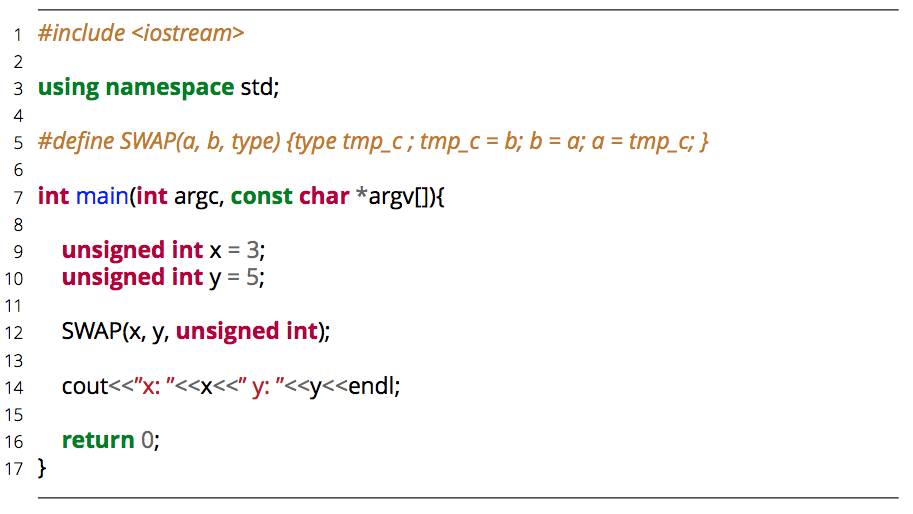
\includegraphics[height=60mm]{/Users/lalanne/MyCode/GitHubProjects/MetaTalk/figures/swap.png}\hspace{5mm}
            };
        \end{tikzpicture}
    \end{center}
\end{frame}

\begin{frame}{C preprocessor SWAP}
    \begin{center}
        \begin{tikzpicture}[]
            \node[] at (0mm,0mm){
                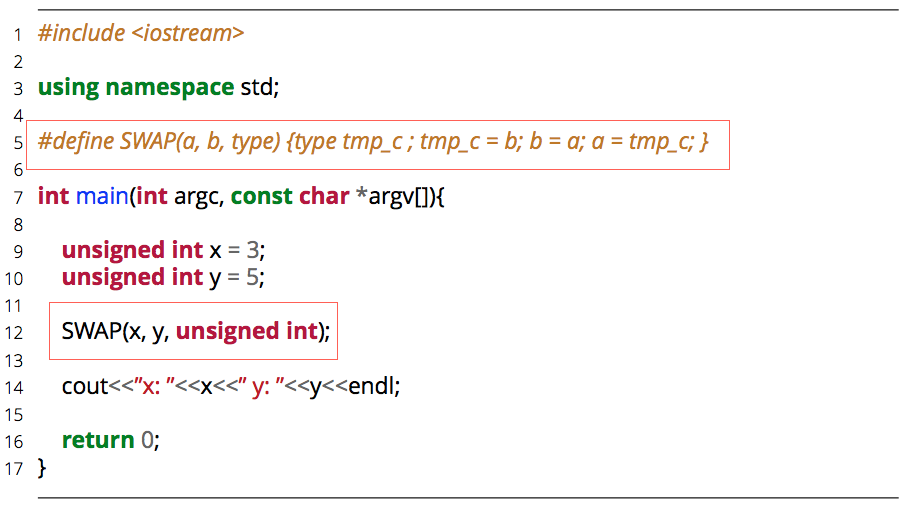
\includegraphics[height=60mm]{/Users/lalanne/MyCode/GitHubProjects/MetaTalk/figures/swap1.png}\hspace{5mm}
            };
        \end{tikzpicture}
    \end{center}
\end{frame}

\begin{frame}{C preprocessor SWAP expanded}
    \begin{center}
        \begin{tikzpicture}[]
            \node[] at (0mm,0mm){
                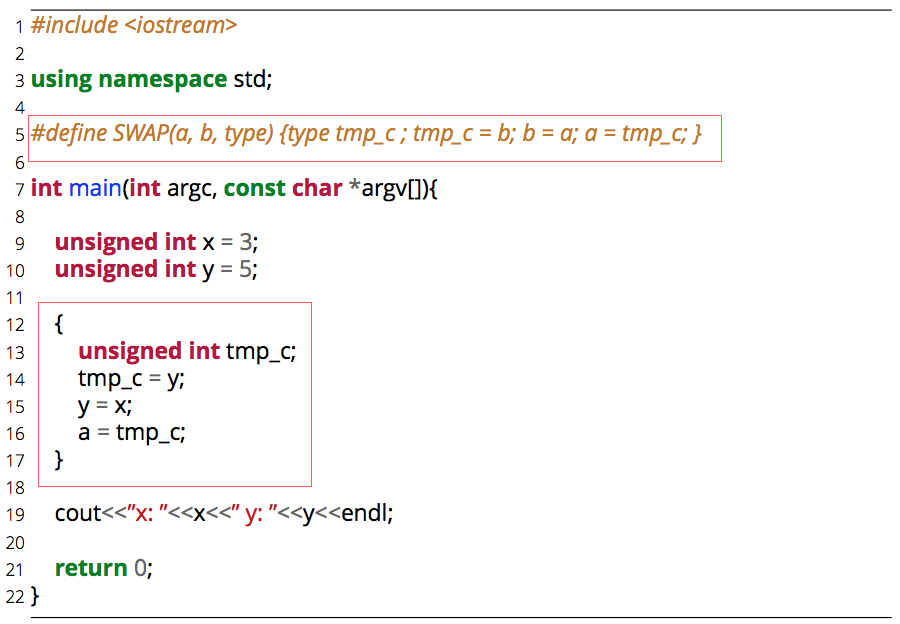
\includegraphics[height=70mm]{/Users/lalanne/MyCode/GitHubProjects/MetaTalk/figures/swapexp1.png}\hspace{5mm}
            };
        \end{tikzpicture}
    \end{center}
\end{frame}

\begin{frame}{C preprocessor SWAP expanded}
    \begin{center}
        \begin{tikzpicture}[]
            \node[] at (0mm,0mm){
                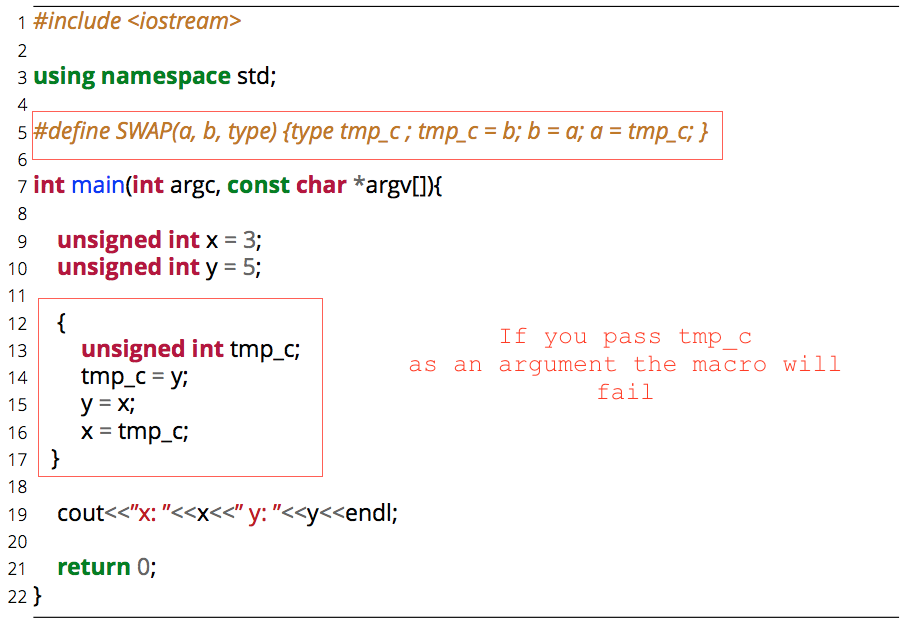
\includegraphics[height=70mm]{/Users/lalanne/MyCode/GitHubProjects/MetaTalk/figures/swapexp2.png}\hspace{5mm}
            };
        \end{tikzpicture}
    \end{center}
\end{frame}


\begin{frame}[fragile]{C preprocessor MIN}
\inputminted[mathescape,
           linenos,
           numbersep=5pt,
           frame=lines,
           bgcolor=White,
           fontsize=\scriptsize,
           linenos,
           framesep=2mm]{c++}
           {/Users/lalanne/MyCode/GitHubProjects/MP_Talk/macro_min.cpp} 
\end{frame}

\begin{frame}[fragile]{C preprocessor MIN}
\inputminted[mathescape,
   linenos,
   numbersep=5pt,
   frame=lines,
   bgcolor=White,
   fontsize=\scriptsize,
   linenos,
   framesep=2mm]{c++}
   {/Users/lalanne/MyCode/GitHubProjects/MetaTalk/src/code/macro_min_fail.cpp} 
\end{frame}

\begin{frame}[fragile]{C preprocessor MIN}
\inputminted[mathescape,
   linenos,
   numbersep=5pt,
   frame=lines,
   bgcolor=White,
   fontsize=\scriptsize,
   linenos,
   framesep=2mm]{c++}
   {/Users/lalanne/MyCode/GitHubProjects/MetaTalk/src/code/macro_min_should.cpp} 
\end{frame}

\begin{frame}[fragile]{C preprocessor MIN}
\inputminted[mathescape,
   linenos,
   numbersep=5pt,
   frame=lines,
   bgcolor=White,
   fontsize=\scriptsize,
   linenos,
   framesep=2mm]{c++}
   {/Users/lalanne/MyCode/GitHubProjects/MetaTalk/src/code/macro_min_res.cpp} 
\end{frame}

\begin{frame}[fragile]{C preprocessor MIN}
\inputminted[mathescape,
   linenos,
   numbersep=5pt,
   frame=lines,
   bgcolor=White,
   fontsize=\scriptsize,
   linenos,
   framesep=2mm]{c++}
   {/Users/lalanne/MyCode/GitHubProjects/MetaTalk/src/code/macro_min_ext.cpp} 
\end{frame}

\begin{frame}{The MIN case}
    \begin{itemize}\addtolength{\itemsep}{2\baselineskip}
        \item Necessary parenthesis (operator precedence), what happen if you 
            do \emph{MIN(27, b=3)}.

        \item When one of the arguments is a function is going to be call twice. 
            (performance, duplicated calculation). Worst when the function
            contains side effects(printing).
    \end{itemize}
\end{frame}

\begin{frame}{Advantages}
    \begin{itemize}\addtolength{\itemsep}{1\baselineskip}
        \item Function call too much overhead for this simple operation (myth).

        \item With big types you end up using pointers(aliasing).
            {\color{red}mmmm check!}

        \item Different functions for different types.
    \end{itemize}
\end{frame}

\begin{frame}{Disadvantages}
    \begin{itemize}\addtolength{\itemsep}{1\baselineskip}
        \item C/C++ preprocessor allow limited arguments for Macros.

        \item You do not get any type of type safety.
            {\color{red} some kind of example of this}

        \item Its get very messy when you combine Macros with expressions.
    \end{itemize}
\end{frame}



\section{C++ Template meta-programming}
\begin{frame}<beamer>                                                                                                                    
    \frametitle{Outline}
    \tableofcontents[currentsection]
\end{frame}
\begin{frame}{C++ Template Meta-programming}
    \begin{itemize}
        \item Templates are used by the compiler to create temporary source code
            \cite{wikiTM}.

        \vspace{5mm}

        \item This code is merge by the compiler with the rest of the source code
            and then compiled\cite{wikiTM}.

        \vspace{5mm}

        \item Compile time execution\cite{wikiTM}.

        \vspace{5mm}

        \item C++, D, Lisp(kind of)\cite{wikiTM}.
    \end{itemize}
\end{frame}

\begin{frame}{Numeric Computations, Compile Time}
    \inputminted[mathescape,                                                       
            linenos,                                                           
            numbersep=5pt,                                                     
            frame=lines,                                                       
            bgcolor=White,                                                     
            fontsize=\scriptsize,                                              
            linenos,                                                           
            framesep=1.5mm]{c++}                                                 
            {/Users/lalanne/MyCode/GitHubProjects/MetaTalk/src/code/basic.cpp}
\end{frame}

\begin{frame}{Numeric Computations, Run Time}
    \inputminted[mathescape,                                                       
    linenos,                                                           
    numbersep=5pt,                                                     
    frame=lines,                                                       
    bgcolor=White,                                                     
    fontsize=\scriptsize,                                              
    linenos,                                                           
    framesep=1.5mm]{c++}                                                 
    {/Users/lalanne/MyCode/GitHubProjects/MetaTalk/src/code/basic_runtime.cpp}
\end{frame}

\begin{frame}{Type Computations}
    \begin{itemize}
        \item This is what has made template metaprogramming in C++ so popular
    \end{itemize}
\end{frame}

\begin{frame}{Type Computations}
    \begin{center}
        \begin{tikzpicture}[]
            \node[] at (0mm,0mm){
                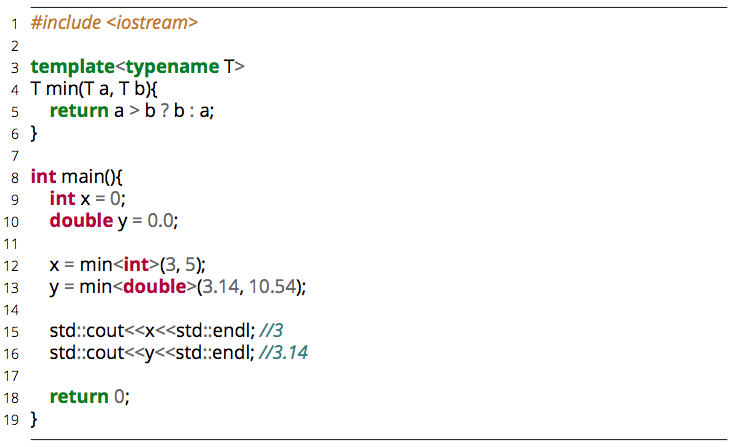
\includegraphics[height=60mm]{/Users/lalanne/MyCode/GitHubProjects/MetaTalk/figures/min_tmp.png}\hspace{5mm}
            };
        \end{tikzpicture}
    \end{center}
\end{frame}

\begin{frame}{Type Computations}
    \begin{center}
        \begin{tikzpicture}[]
            \node[] at (0mm,0mm){
                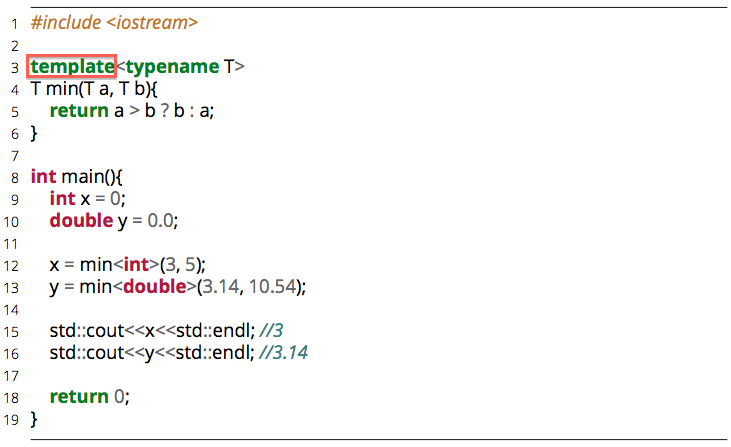
\includegraphics[height=60mm]{/Users/lalanne/MyCode/GitHubProjects/MetaTalk/figures/min_tmp_1.png}\hspace{5mm}
            };
        \end{tikzpicture}
    \end{center}
\end{frame}

\begin{frame}{Type Computations}
    \begin{center}
        \begin{tikzpicture}[]
            \node[] at (0mm,0mm){
                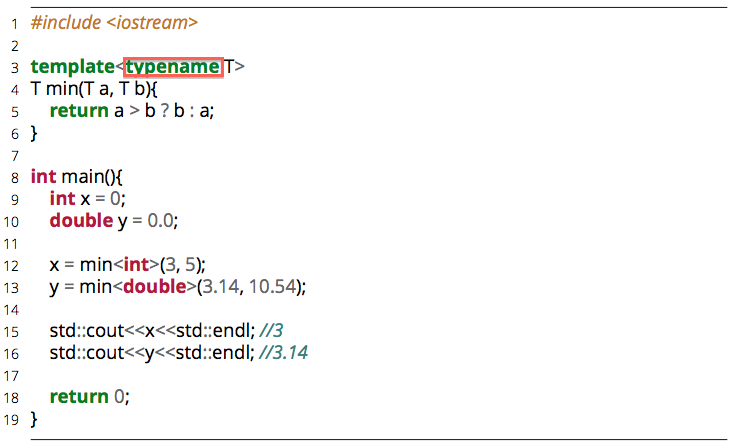
\includegraphics[height=60mm]{/Users/lalanne/MyCode/GitHubProjects/MetaTalk/figures/min_tmp_2.png}\hspace{5mm}
            };
        \end{tikzpicture}
    \end{center}
\end{frame}

\begin{frame}{Type Computations}
    \begin{center}
        \begin{tikzpicture}[]
            \node[] at (0mm,0mm){
                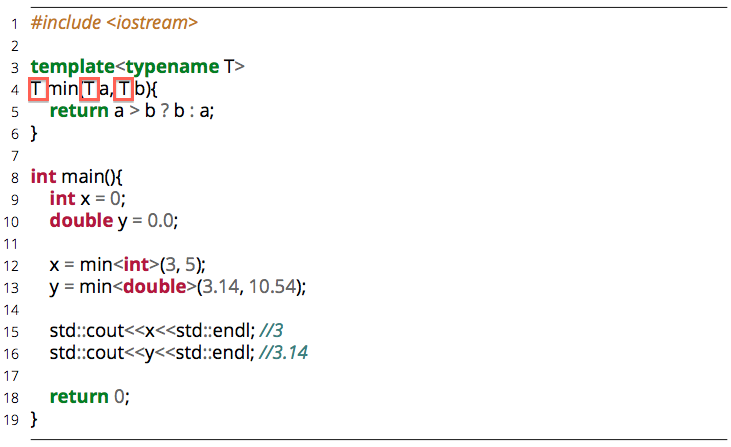
\includegraphics[height=60mm]{/Users/lalanne/MyCode/GitHubProjects/MetaTalk/figures/min_tmp_3.png}\hspace{5mm}
            };
        \end{tikzpicture}
    \end{center}
\end{frame}

\begin{frame}{Type Computations}
    \begin{center}
        \begin{tikzpicture}[]
            \node[] at (0mm,0mm){
                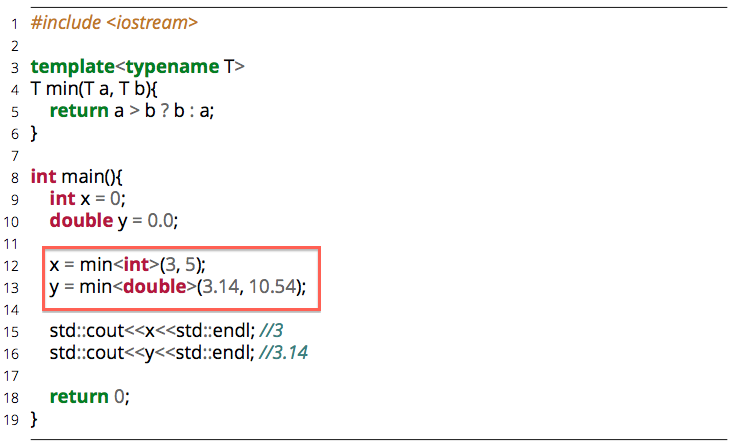
\includegraphics[height=60mm]{/Users/lalanne/MyCode/GitHubProjects/MetaTalk/figures/min_tmp_4.png}\hspace{5mm}
            };
        \end{tikzpicture}
    \end{center}
\end{frame}

\begin{frame}{Type Computations}
    \begin{center}
        \begin{tikzpicture}[]
            \node[] at (0mm,0mm){
                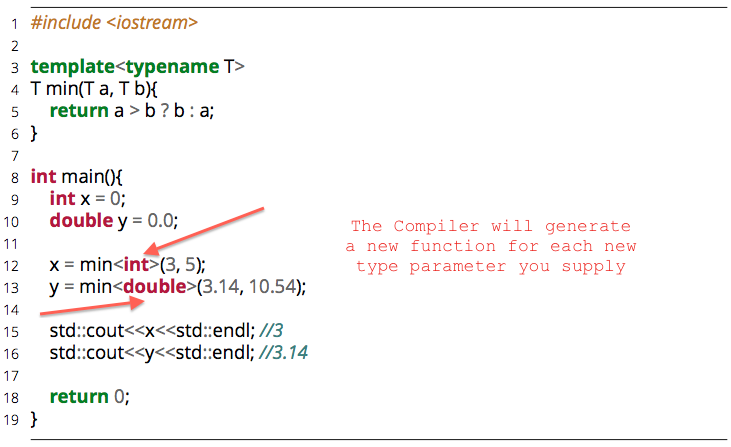
\includegraphics[height=60mm]{/Users/lalanne/MyCode/GitHubProjects/MetaTalk/figures/min_tmp_5.png}\hspace{5mm}
            };
        \end{tikzpicture}
    \end{center}
\end{frame}

\begin{frame}{Type Computations}
    \begin{center}
        \begin{tikzpicture}[]
            \node[] at (0mm,0mm){
                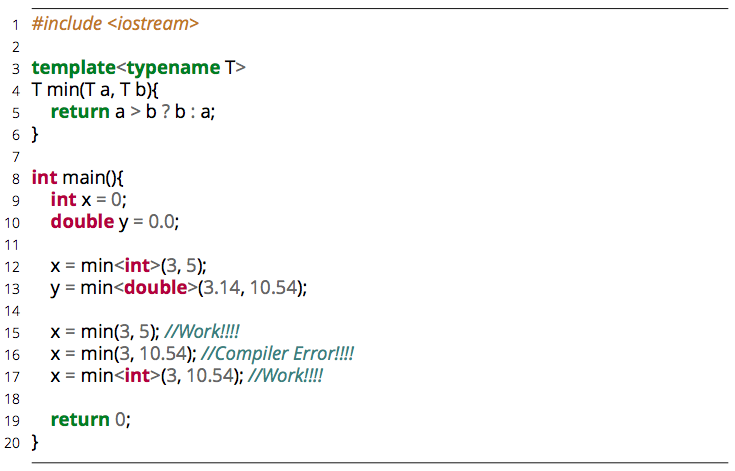
\includegraphics[height=60mm]{/Users/lalanne/MyCode/GitHubProjects/MetaTalk/figures/min_comp_types.png}\hspace{5mm}
            };
        \end{tikzpicture}
    \end{center}
\end{frame}

\begin{frame}{Type Computations}
    \begin{center}
        \begin{tikzpicture}[]
            \node[] at (0mm,0mm){
                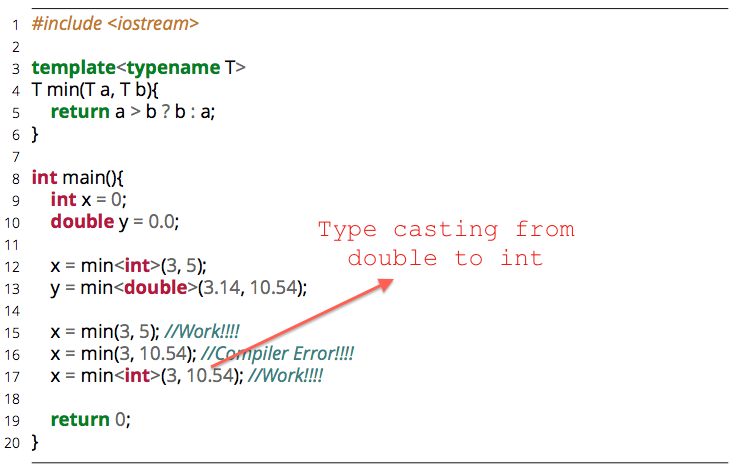
\includegraphics[height=60mm]{/Users/lalanne/MyCode/GitHubProjects/MetaTalk/figures/min_comp_types_1.png}\hspace{5mm}
            };
        \end{tikzpicture}
    \end{center}
\end{frame}

\begin{frame}[t]{Type Computations}
    \begin{itemize}
        \item New code is generated for each new type that the compiler encounters
        \item A template instance is only created once
        \item Multiple calls use the same object code created
    \end{itemize}
    \begin{center}
        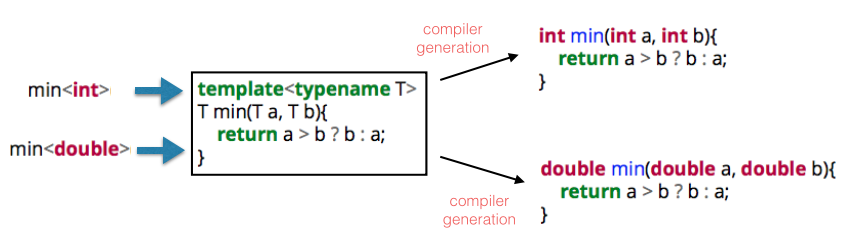
\includegraphics[height=30mm]{/Users/lalanne/MyCode/GitHubProjects/MetaTalk/figures/scheme.png}
    \end{center}
\end{frame}








\section{Design Patterns}
\begin{frame}<beamer>                                                                                                                    
    \frametitle{Outline}
    \tableofcontents[currentsection]
\end{frame}
\begin{frame}{Design Patterns}                                                                                                              
\begin{itemize}
\item .
\end{itemize}
\end{frame}


\section{Erasing virtual methods}
\subsection{Virtual Tables}
\begin{frame}{Dynamic Dispatching}
    \begin{itemize}
        \item When designing a system you usually know which kind of interface
            do you want but not the concrete implementation
        \item The goal is to reduce the effort in changing implementations
        \item \textbf{Dynamic Dispatching:} Which mplementation of a 
            method(class function) to call at run-time
    \end{itemize}
\end{frame}

\begin{frame}[fragile]{Dynamic Dispatching, How does it look like?}
    \begin{columns}[T]
        \begin{column}[T]{5cm}
            \inputminted[mathescape,
                       linenos,
                       numbersep=2pt,
                       frame=lines,
                       bgcolor=White,
                       fontsize=\tiny,
                       linenos,
                       framesep=1mm]{c++}
                       {/Users/lalanne/MyCode/GitHubProjects/MetaTalk/src/code/dd_1.cpp} 
        \end{column}
        \begin{column}[T]{5cm}
            \inputminted[mathescape,
                   linenos,
                   numbersep=2pt,
                   frame=lines,
                   bgcolor=White,
                   fontsize=\tiny,
                   linenos,
                   framesep=1mm]{c++}
                   {/Users/lalanne/MyCode/GitHubProjects/MetaTalk/src/code/dd_2.cpp}
        \end{column}
    \end{columns}
\end{frame}

\begin{frame}{Virtual Functions}
    \begin{center}
        \begin{tikzpicture}[]
            \node[] at (0mm,0mm){
                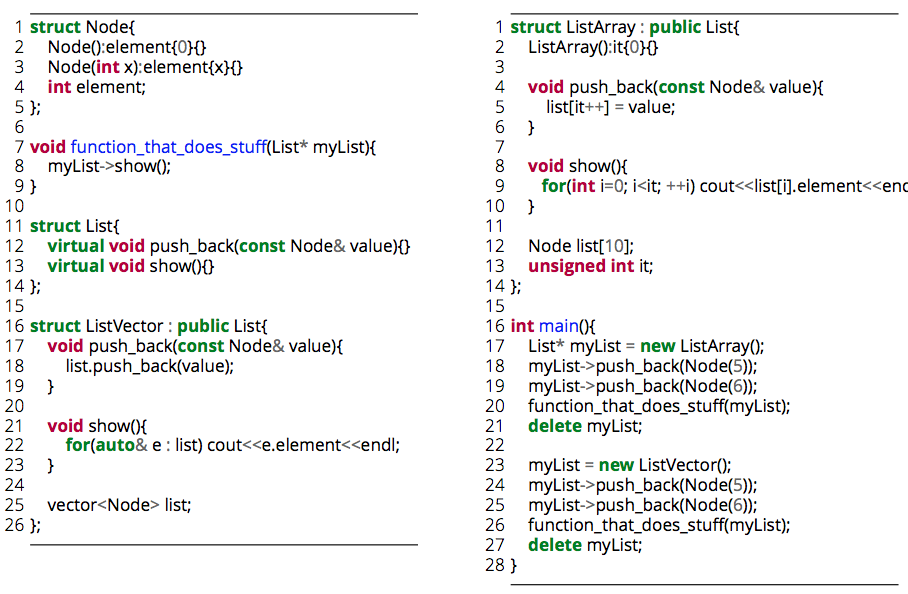
\includegraphics[height=70mm]{/Users/lalanne/MyCode/GitHubProjects/MetaTalk/figures/ddp1.png}\hspace{5mm}
            };
        \end{tikzpicture}
    \end{center}
\end{frame}

\begin{frame}{Virtual Functions}
    \begin{center}
        \begin{tikzpicture}[]
            \node[] at (0mm,0mm){
                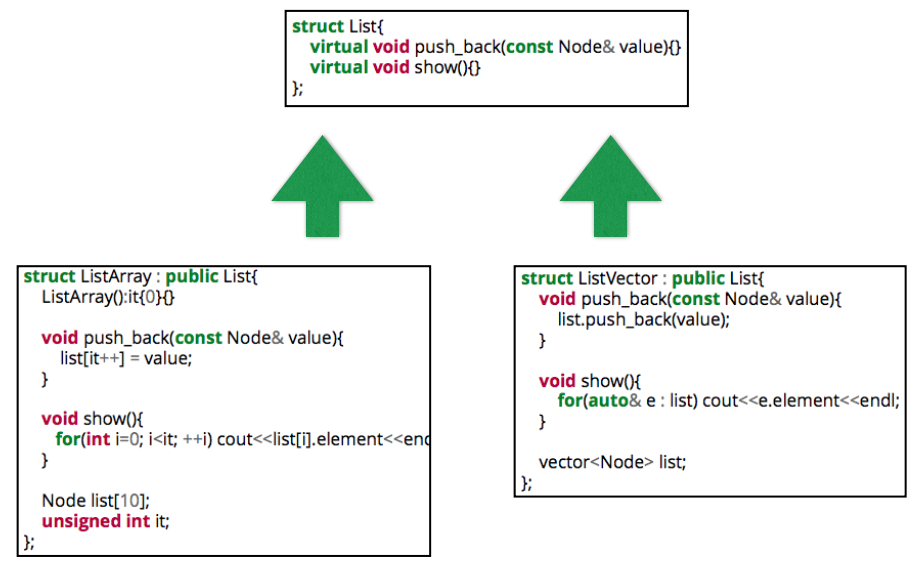
\includegraphics[height=70mm]{/Users/lalanne/MyCode/GitHubProjects/MetaTalk/figures/classdiag.png}\hspace{5mm}
            };
        \end{tikzpicture}
    \end{center}
\end{frame}

\begin{frame}{Virtual Functions}
    \begin{center}
        \begin{tikzpicture}[]
            \node[] at (0mm,0mm){
                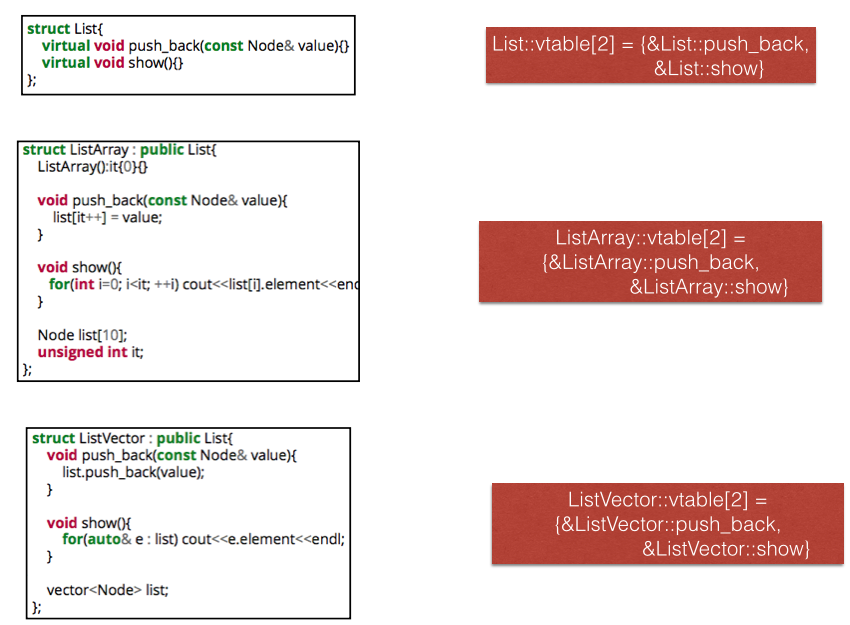
\includegraphics[height=70mm]{/Users/lalanne/MyCode/GitHubProjects/MetaTalk/figures/vtbl1.png}\hspace{5mm}
            };
        \end{tikzpicture}
    \end{center}
\end{frame}

\begin{frame}{Virtual Functions}
    \begin{center}
        \begin{tikzpicture}[]
            \node[] at (0mm,0mm){
                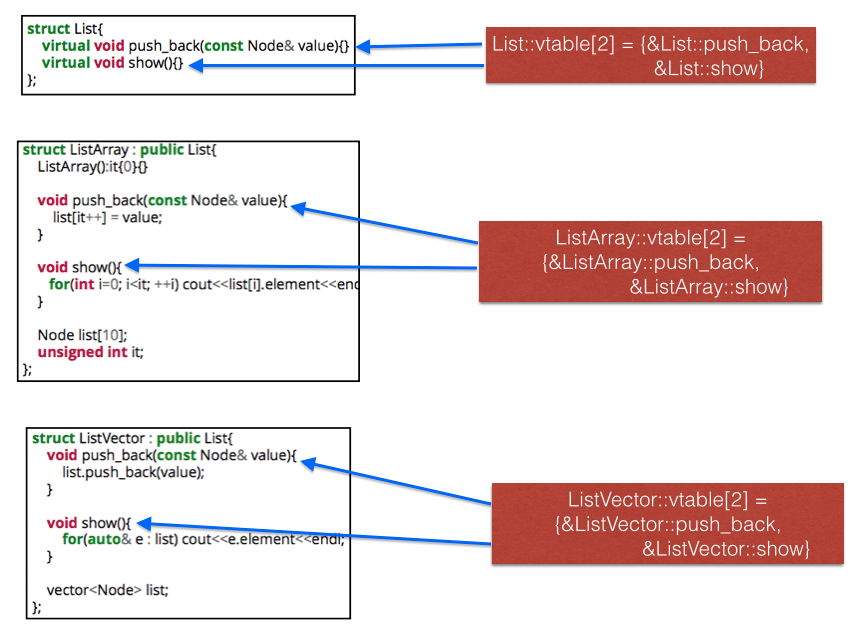
\includegraphics[height=70mm]{/Users/lalanne/MyCode/GitHubProjects/MetaTalk/figures/vtbl1_1.png}\hspace{5mm}
            };
        \end{tikzpicture}
    \end{center}
\end{frame}

\begin{frame}{Virtual Functions}
    \begin{center}
        \begin{tikzpicture}[]
            \node[] at (0mm,0mm){
                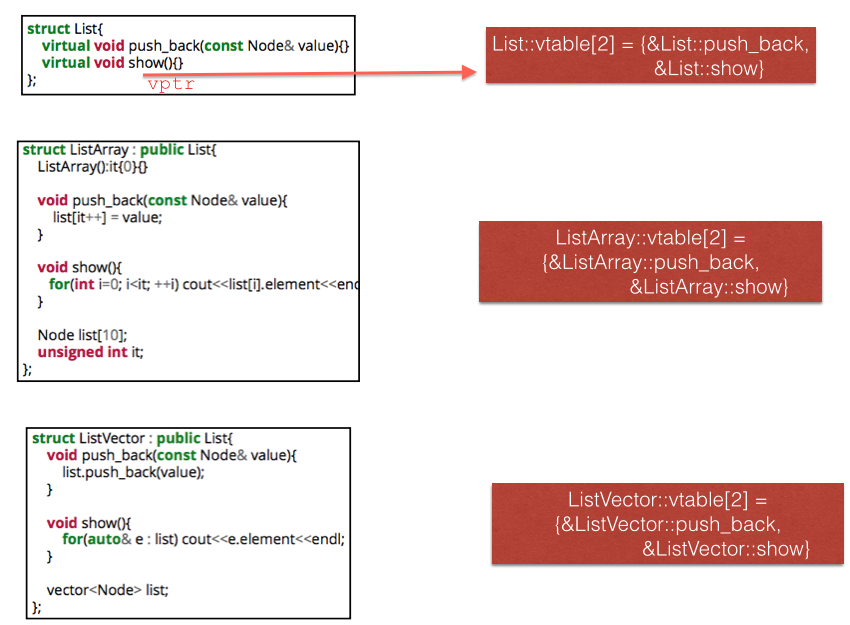
\includegraphics[height=70mm]{/Users/lalanne/MyCode/GitHubProjects/MetaTalk/figures/vtbl2.png}\hspace{5mm}
            };
        \end{tikzpicture}
    \end{center}
\end{frame}

\begin{frame}{Virtual Functions}
    \begin{center}
        \begin{tikzpicture}[]
            \node[] at (0mm,0mm){
                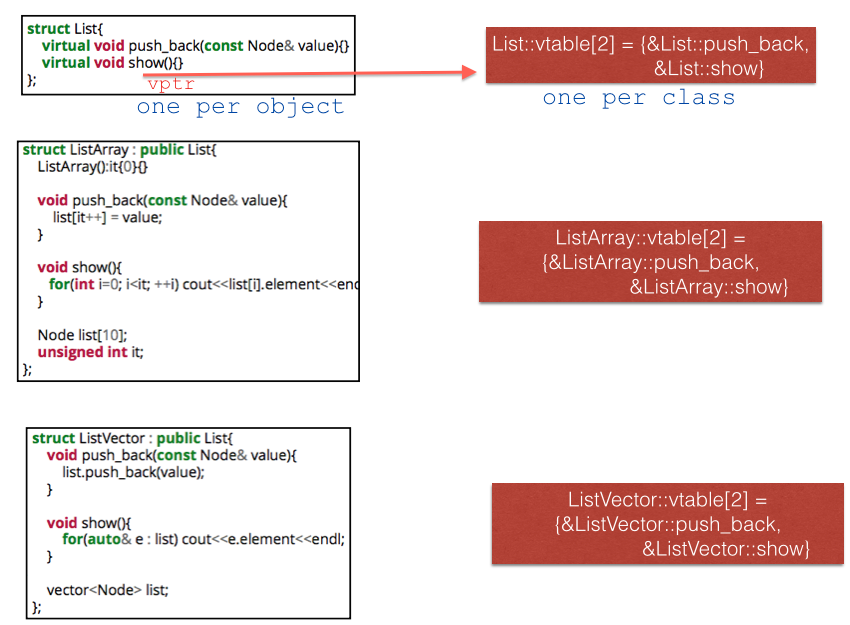
\includegraphics[height=70mm]{/Users/lalanne/MyCode/GitHubProjects/MetaTalk/figures/vtbl3.png}\hspace{5mm}
            };
        \end{tikzpicture}
    \end{center}
\end{frame}

\begin{frame}{Virtual Functions}
    \begin{center}
        \begin{tikzpicture}[]
            \node[] at (0mm,0mm){
                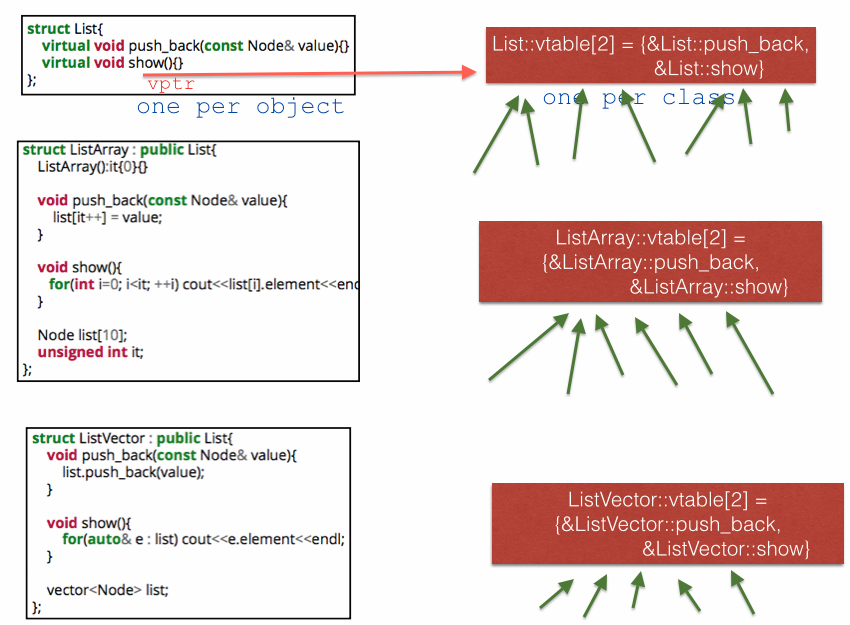
\includegraphics[height=70mm]{/Users/lalanne/MyCode/GitHubProjects/MetaTalk/figures/vtbl3_1.png}\hspace{5mm}
            };
        \end{tikzpicture}
    \end{center}
\end{frame}

\begin{frame}{Virtual Functions}
    \begin{center}
        \begin{tikzpicture}[]
            \node[] at (0mm,0mm){
                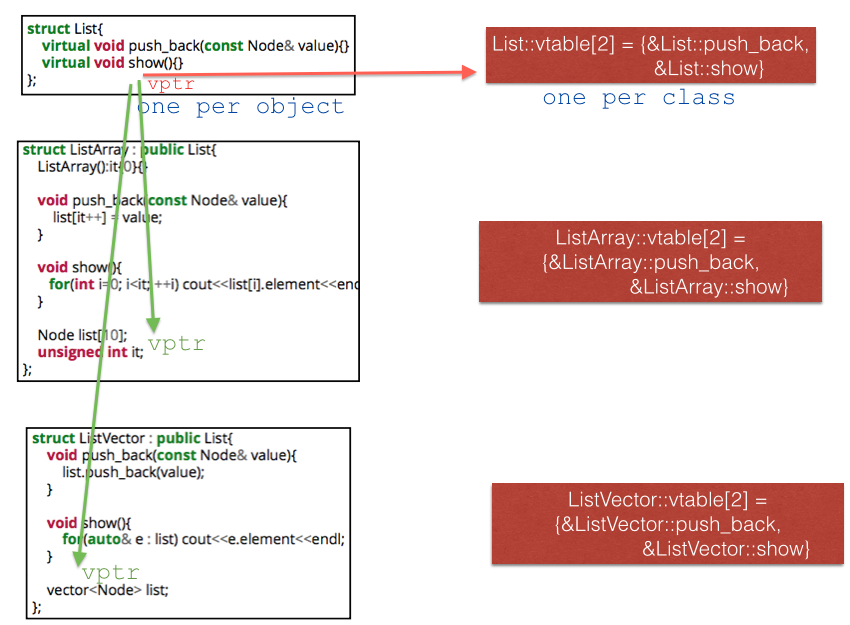
\includegraphics[height=70mm]{/Users/lalanne/MyCode/GitHubProjects/MetaTalk/figures/vtbl4.png}\hspace{5mm}
            };
        \end{tikzpicture}
    \end{center}
\end{frame}


\begin{frame}{Virtual Functions}
    \begin{center}
        \begin{tikzpicture}[]
            \node[] at (0mm,0mm){
                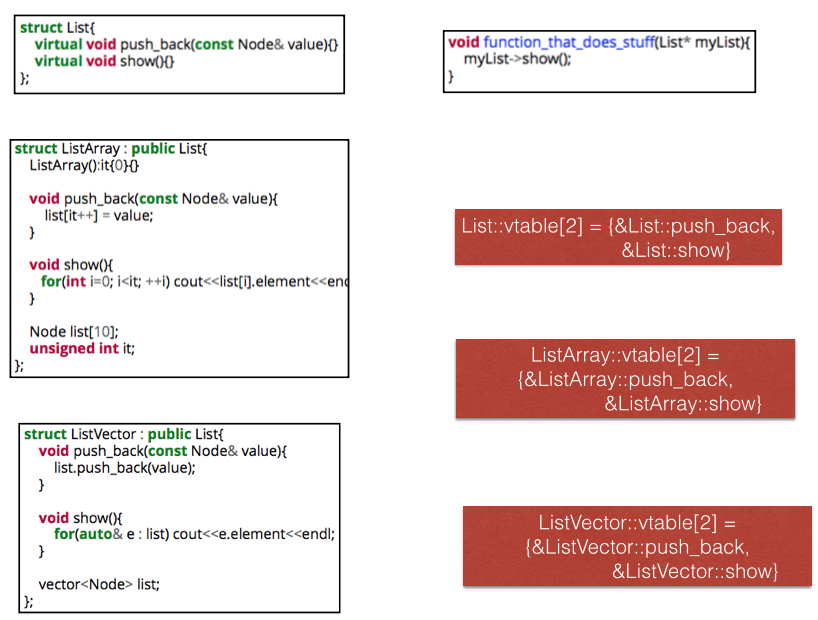
\includegraphics[height=70mm]{/Users/lalanne/MyCode/GitHubProjects/MetaTalk/figures/vtblpluscall.png}\hspace{5mm}
            };
        \end{tikzpicture}
    \end{center}
\end{frame}

\begin{frame}{Virtual Functions}
    \begin{center}
        \begin{tikzpicture}[]
            \node[] at (0mm,0mm){
                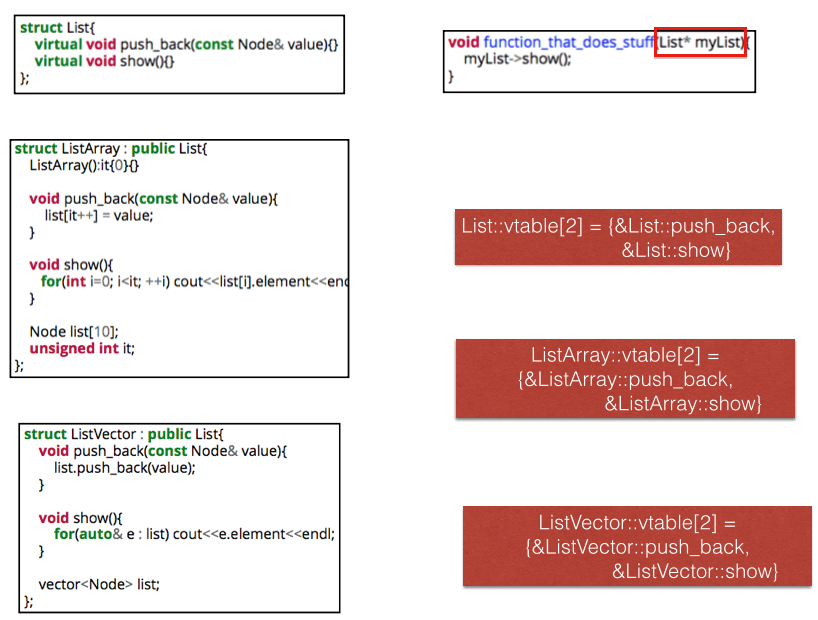
\includegraphics[height=70mm]{/Users/lalanne/MyCode/GitHubProjects/MetaTalk/figures/vtblpluscall1.png}\hspace{5mm}
            };
        \end{tikzpicture}
    \end{center}
\end{frame}

\begin{frame}{Virtual Functions}
    \begin{center}
        \begin{tikzpicture}[]
            \node[] at (0mm,0mm){
                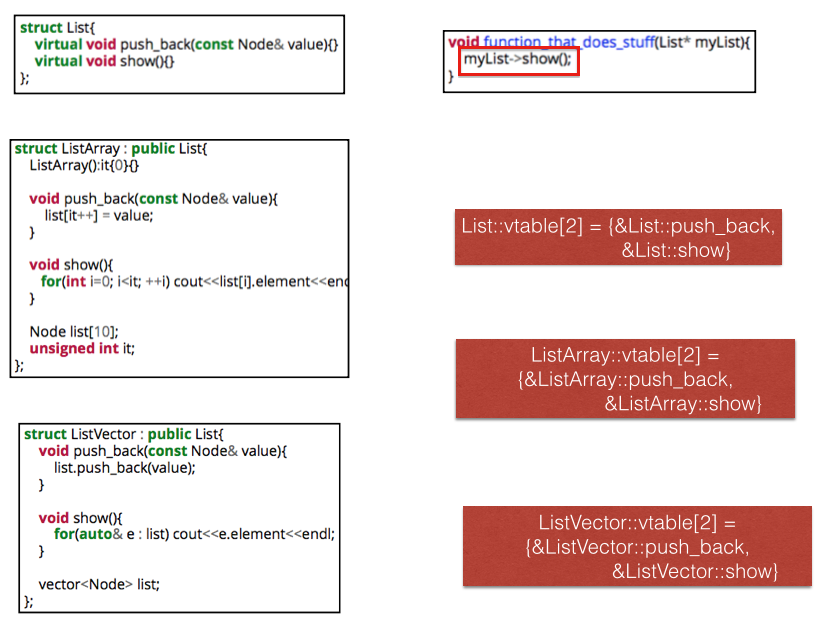
\includegraphics[height=70mm]{/Users/lalanne/MyCode/GitHubProjects/MetaTalk/figures/vtblpluscall2.png}\hspace{5mm}
            };
        \end{tikzpicture}
    \end{center}
\end{frame}

\begin{frame}{Virtual Functions}
    \begin{center}
        \begin{tikzpicture}[]
            \node[] at (0mm,0mm){
                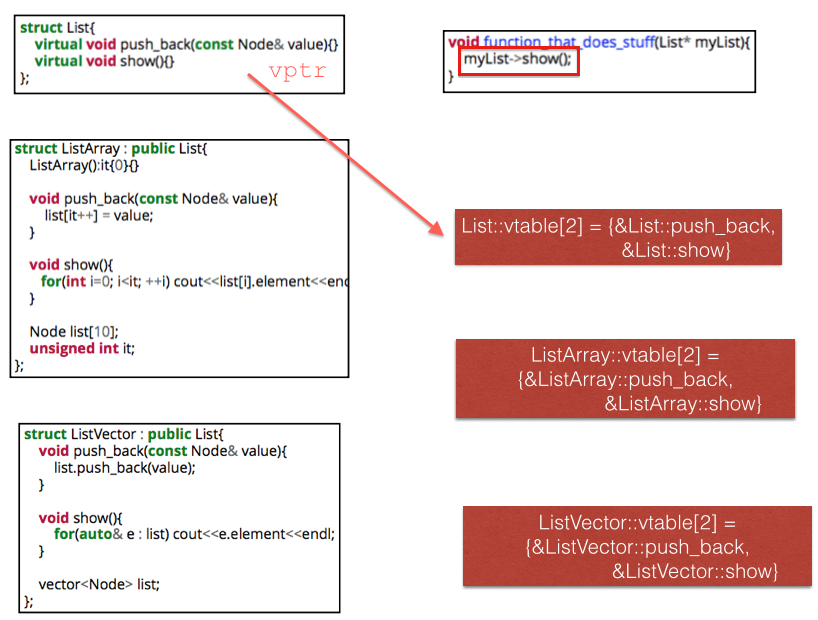
\includegraphics[height=70mm]{/Users/lalanne/MyCode/GitHubProjects/MetaTalk/figures/vtblpluscall3.png}\hspace{5mm}
            };
        \end{tikzpicture}
    \end{center}
\end{frame}

\begin{frame}{Virtual Functions}
    \begin{center}
        \begin{tikzpicture}[]
            \node[] at (0mm,0mm){
                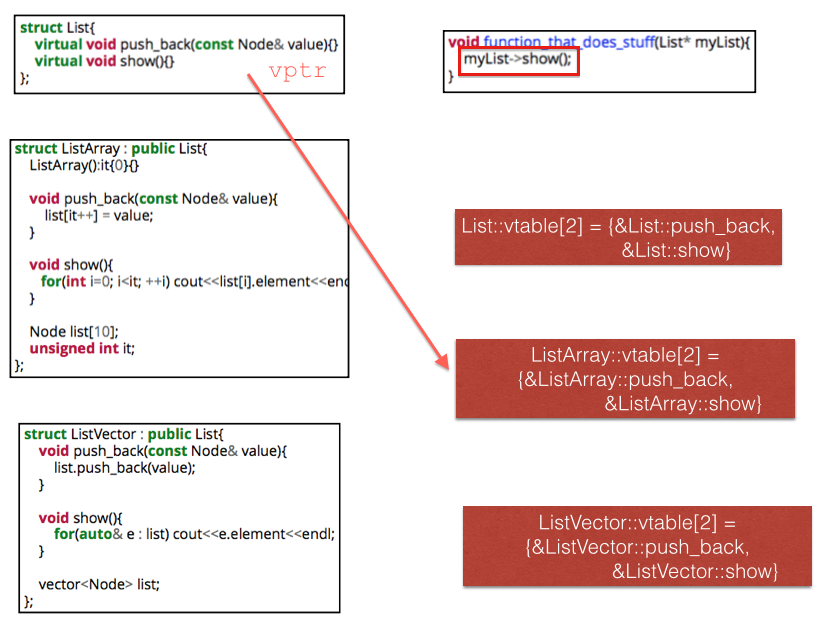
\includegraphics[height=70mm]{/Users/lalanne/MyCode/GitHubProjects/MetaTalk/figures/vtblpluscall4.png}\hspace{5mm}
            };
        \end{tikzpicture}
    \end{center}
\end{frame}

\begin{frame}{Virtual Functions}
    \begin{center}
        \begin{tikzpicture}[]
            \node[] at (0mm,0mm){
                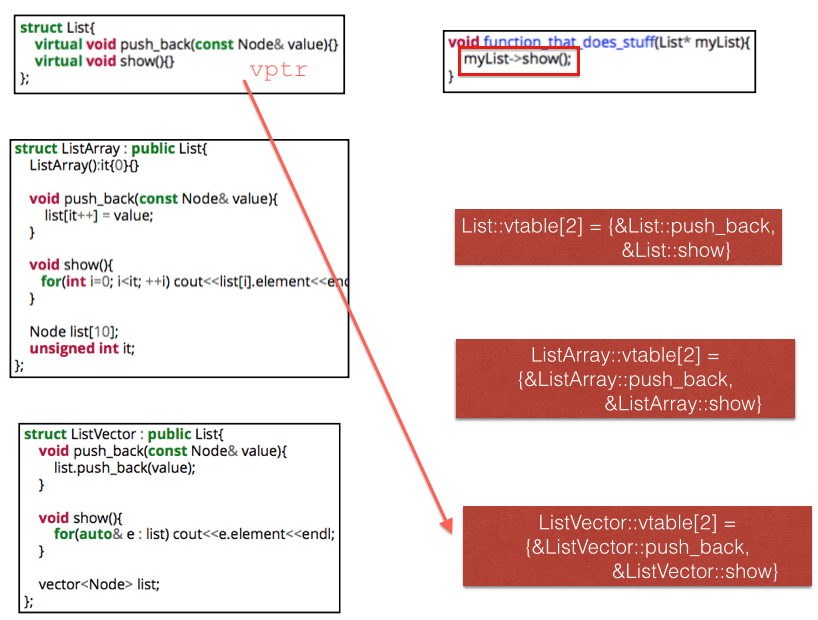
\includegraphics[height=70mm]{/Users/lalanne/MyCode/GitHubProjects/MetaTalk/figures/vtblpluscall5.png}\hspace{5mm}
            };
        \end{tikzpicture}
    \end{center}
\end{frame}

\begin{frame}{Virtual Functions}
    \begin{itemize}
        \item First load \emph{vptr} to register (r1)
        \item Second load \emph{vptr + offset} to register (r2)
        \item Call function (r2)
    \end{itemize}

    \begin{itemize}
        \item Small size overhead(think small classes)
        \item Call overhead
    \end{itemize}
\end{frame}


\subsection{naive}
\begin{frame}{Erasing virtual methods, naive} 
    \begin{itemize}
        \item .
    \end{itemize}
\end{frame}

\subsection{crtp}
\begin{frame}[Generate]{Erasing virtual methods, CRTP} 
\begin{itemize}
\item Curiously Recurring Template Pattern.
\item \cite{eli}
\end{itemize}
\end{frame}

\begin{frame}[fragile]{CRTP, run time polymorphism}
\inputminted[mathescape,
           linenos,
           numbersep=5pt,
           frame=lines,
           bgcolor=White,
           fontsize=\tiny,
           linenos,
           framesep=2mm]{c++}
           {/Users/lalanne/MyCode/GitHubProjects/MetaTalk/src/code/run_complex_pol_mine_1.cpp} 
\end{frame}

\begin{frame}[fragile]{CRTP, run time polymorphism}
\inputminted[mathescape,
           linenos,
           numbersep=5pt,
           frame=lines,
           bgcolor=White,
           fontsize=\scriptsize,
           linenos,
           framesep=2mm]{c++}
           {/Users/lalanne/MyCode/GitHubProjects/MetaTalk/src/code/run_complex_pol_mine_2.cpp} 
\end{frame}

\begin{frame}[fragile]{CRTP, compile time polymorphism}
\inputminted[mathescape,
           linenos,
           numbersep=5pt,
           frame=lines,
           bgcolor=White,
           fontsize=\tiny,
           linenos,
           framesep=2mm]{c++}
           {/Users/lalanne/MyCode/GitHubProjects/MetaTalk/src/code/comp_complex_pol_mine_1.cpp} 
\end{frame}

\begin{frame}[fragile]{CRTP, compile time polymorphism}
\inputminted[mathescape,
           linenos,
           numbersep=5pt,
           frame=lines,
           bgcolor=White,
           fontsize=\scriptsize,
           linenos,
           framesep=2mm]{c++}
           {/Users/lalanne/MyCode/GitHubProjects/MetaTalk/src/code/comp_complex_pol_mine_2.cpp} 
\end{frame}

\begin{frame}[fragile]{CRTP, compile time polymorphism}
\inputminted[mathescape,
           linenos,
           numbersep=5pt,
           frame=lines,
           bgcolor=White,
           fontsize=\scriptsize,
           linenos,
           framesep=2mm]{c++}
           {/Users/lalanne/MyCode/GitHubProjects/MetaTalk/src/code/comp_complex_pol_mine_3.cpp} 
\end{frame}


\begin{frame}[fragile]{CRTP, compile time polymorphism}
    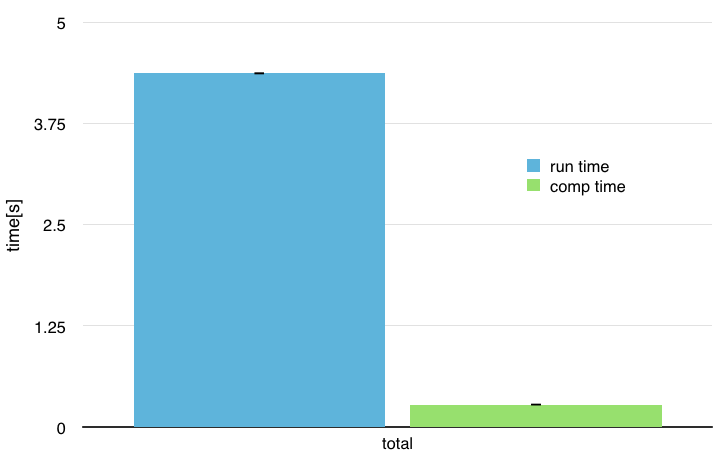
\includegraphics[scale=0.3]{/Users/lalanne/MyCode/GitHubProjects/MetaTalk/figures/crt.png}
\end{frame}

\begin{frame}[fragile]{Logical CPU balance}
\vspace{20mm}
\begin{figure}
\begin{tikzpicture}[font=\footnotesize,xshift=-25mm,yshift=-17mm]
\begin{axis}[
ybar,
xtick=data,
scale only axis,
xticklabels={A, B},
minor tick num =4,
every tick/.style={thick},
ylabel=seconds,
width=0.55\textwidth,
]
\addplot +[blue,thick] table[x index=0, y index=  1] {/Users/lalanne/MyCode/GitHubProjects/MetaTalk/figures/vtune.dat};
\end{axis}
\end{tikzpicture}
\end{figure}
\vspace{20mm}
\par{}
\end{frame}



\section{Gilles example}
\begin{frame}<beamer>                                                                                                                    
    \frametitle{Outline}
    \tableofcontents[currentsection]
\end{frame}
\begin{frame}{Gilles Example}                                                                                                              
\begin{itemize}
\item .
\end{itemize}
\end{frame}


\section{Expression Templates:}
\begin{frame}<beamer>                                                                                                                    
    \frametitle{Outline}
    \tableofcontents[currentsection]
\end{frame}
\begin{frame}{Expression Templates}                                                                                                              
\begin{itemize}
\item .
\end{itemize}
\end{frame}


\section{References}

\begin{frame}[allowframebreaks]
  \frametitle<presentation>{References}    

  \begin{thebibliography}{5}    
  \beamertemplatebookbibitems
  \bibitem{AbrahamsAndGurtovoy04}
    David Abrahams and Aleksey Gurtovoy 2004.
    \newblock {\em C++ Template Metaprogramming, Concepts, Tools and Techniques from Boost and Beyond.}

  \beamertemplatearticlebibitems
  \bibitem{Jemand2000}
    S.~Jemand.
    \newblock On this and that.
    \newblock {\em Journal of This and That}, 2(1):50--100, 2000.

  \setbeamertemplate{bibliography item}[online]
  \bibitem{macrosibm} 
    Jonathan Bartlett 2005.
    \newblock{\em The art of metaprogramming, Part 1: Introduction to metaprogramming.}
    \newblock{\em http://www.ibm.com/developerworks/library/l-metaprog1/}

  \setbeamertemplate{bibliography item}[online]
  \bibitem{wikiTM} 
    Wikipedia.
    \newblock{\em Template Metaprogramming.}
    \newblock{\em http://en.wikipedia.org/wiki/Template\_metaprogramming}

  \setbeamertemplate{bibliography item}[online]
  \bibitem{eli} 
    Eli Bendersky 2013.
    \newblock{\em The cost of dynamic(virtual calls) vs. static(CRTP) dispatch in C++.}
    \newblock{\em http://eli.thegreenplace.net/2013/12/05/the-cost-of-dynamic-virtual-calls-vs-static-crtp-dispatch-in-c/}
  \end{thebibliography}

\end{frame}

\section*{Questions}
\begin{frame}{Q\&A}
 \begin{center}
   \begin{tikzpicture}[]
     \node[] at (0mm,0mm){
       
\includegraphics[height=30mm]{questionR.jpg}\hspace{5mm}
       
\includegraphics[height=30mm]{questionB.jpg}\hspace{5mm}
       
\includegraphics[height=30mm]{questionW.png}
     };
   \end{tikzpicture}
 \end{center}
\addtocounter{framenumber}{-1}
\note<+->{.}
\end{frame}
\end{document}
